\chapter{Конструкторская часть}

В данном разделе будут представлены требования к программному обеспечению и схемы рассматриваемых алгоритмов.

\section{Требования к программному обеспечению}

К программе предъявлены ряд требований:

\begin{itemize}
	\item наличие меню для выбора запускаемого режима работы конвейера --- последовательного или параллельного;
	\item предоставление интерфейса для ввода числа заявок;
	\item формирование файла с результатами журналирования работы конвейера.
\end{itemize}

\section{Разработка алгоритмов}

На рисунке~\ref{lin} представлен последовательный алгоритм работы стадий конвейера.

\begin{figure}[h]
	\centering
	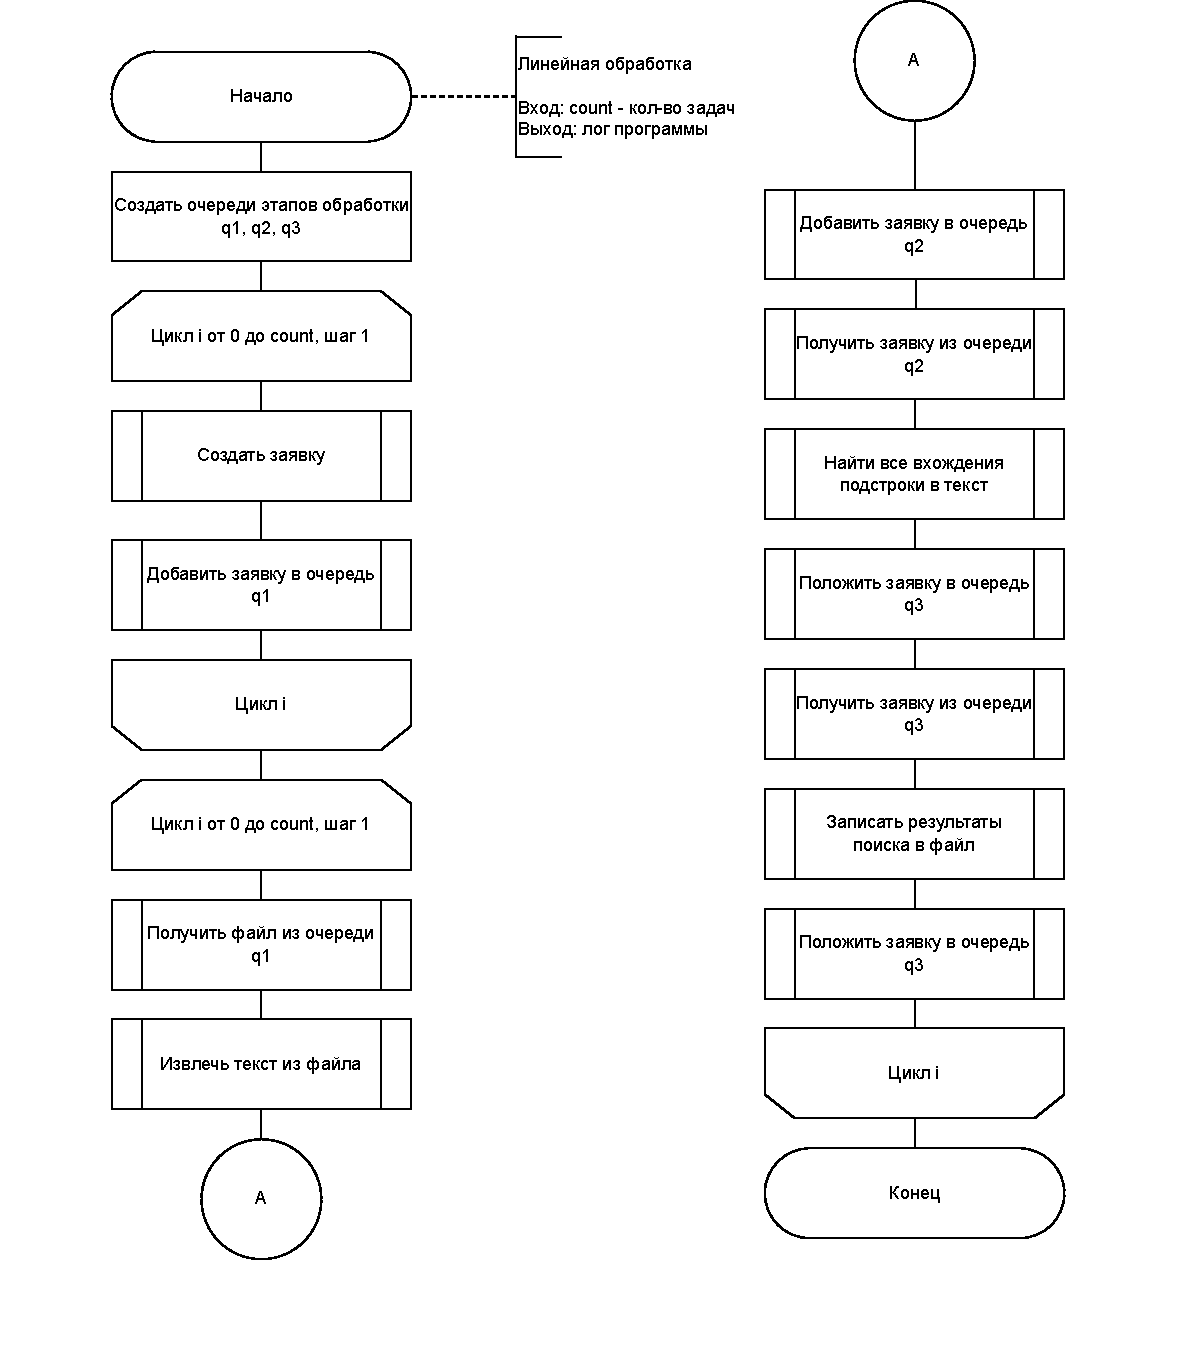
\includegraphics[scale=0.9]{photos/linear}
	\caption{Схема алгоритма последовательной конвейерной обработки}
	\label{lin}
\end{figure}
\clearpage

Параллельная работа будет реализована с помощью добавления 3-х
вспомогательных потоков, где каждый поток отвечает за свою стадию обработки.

На рисунке~\ref{paral} представлена схема главного потока при параллельной
работе стадий конвейера.

\begin{figure}[h]
	\centering
	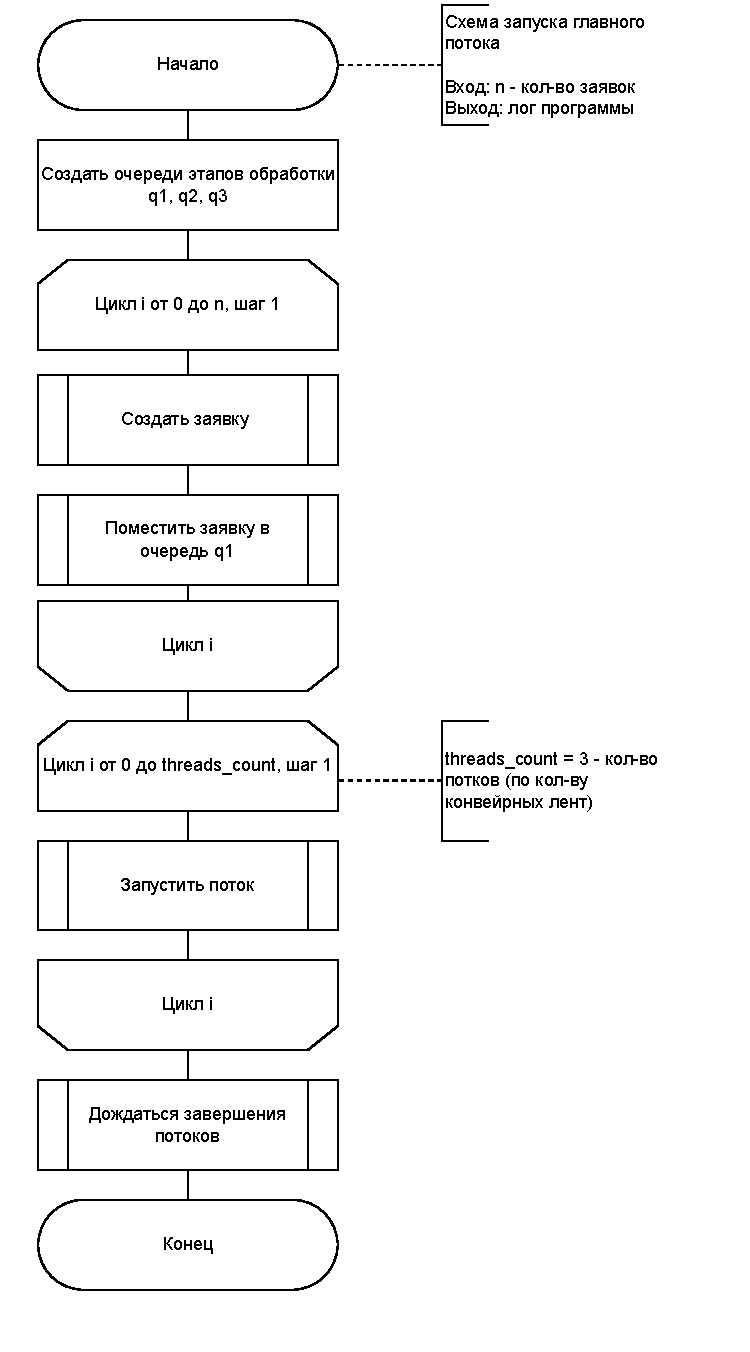
\includegraphics[scale=0.8]{photos/main_thread}
	\caption{Схема главного потока при параллельной работе конвейера}
	\label{paral}
\end{figure}
\clearpage

На рисунках~\ref{sh1}, ~\ref{sh2} и~\ref{sh3} представлены схемы алгоритмов каждого из обработчиков (потоков) при параллельной работе.

\begin{figure}[h]
	\centering
	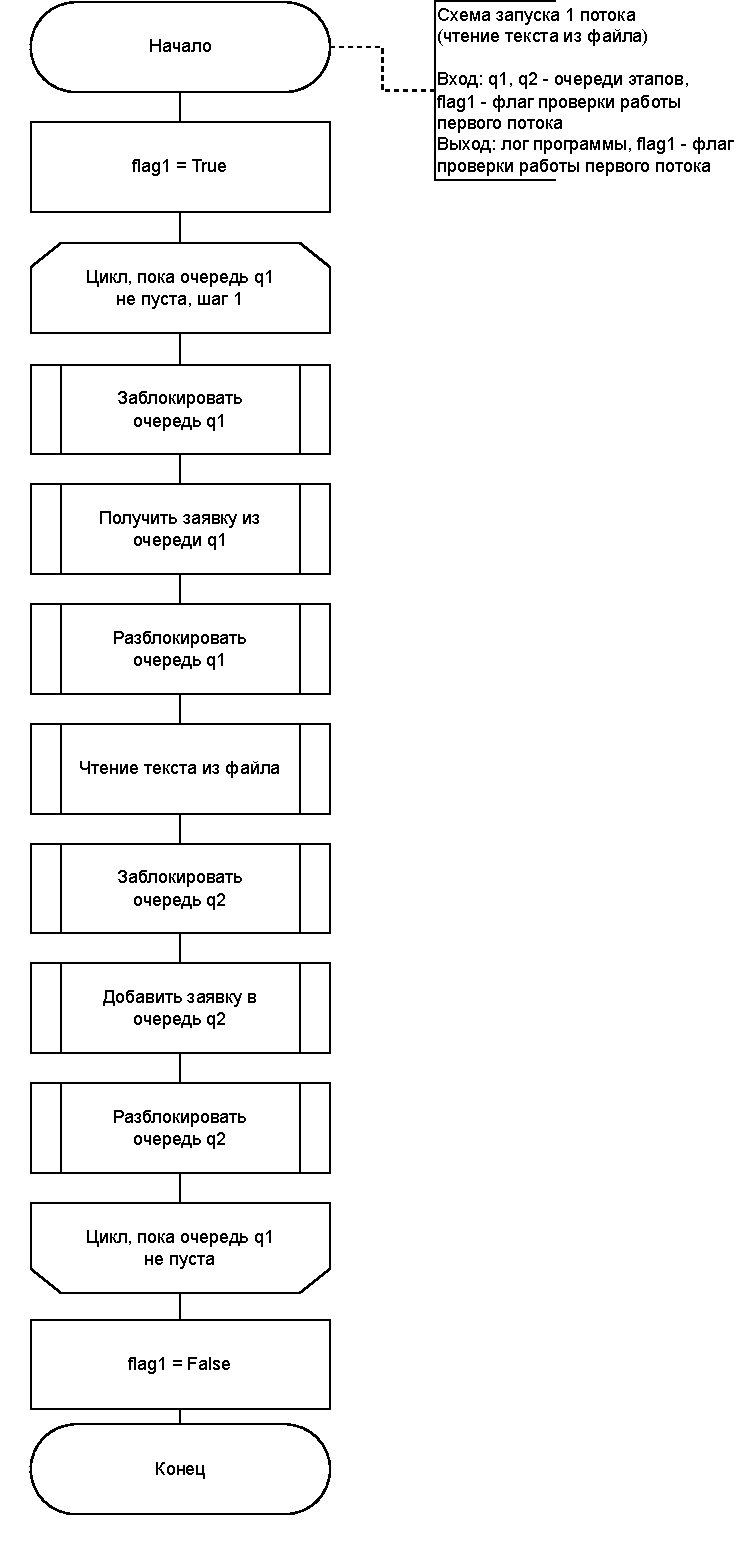
\includegraphics[scale=0.72]{photos/thread1}
	\caption{Схема алгоритма потока 1}
	\label{sh1}
\end{figure}
\clearpage

\begin{figure}[h]
	\centering
	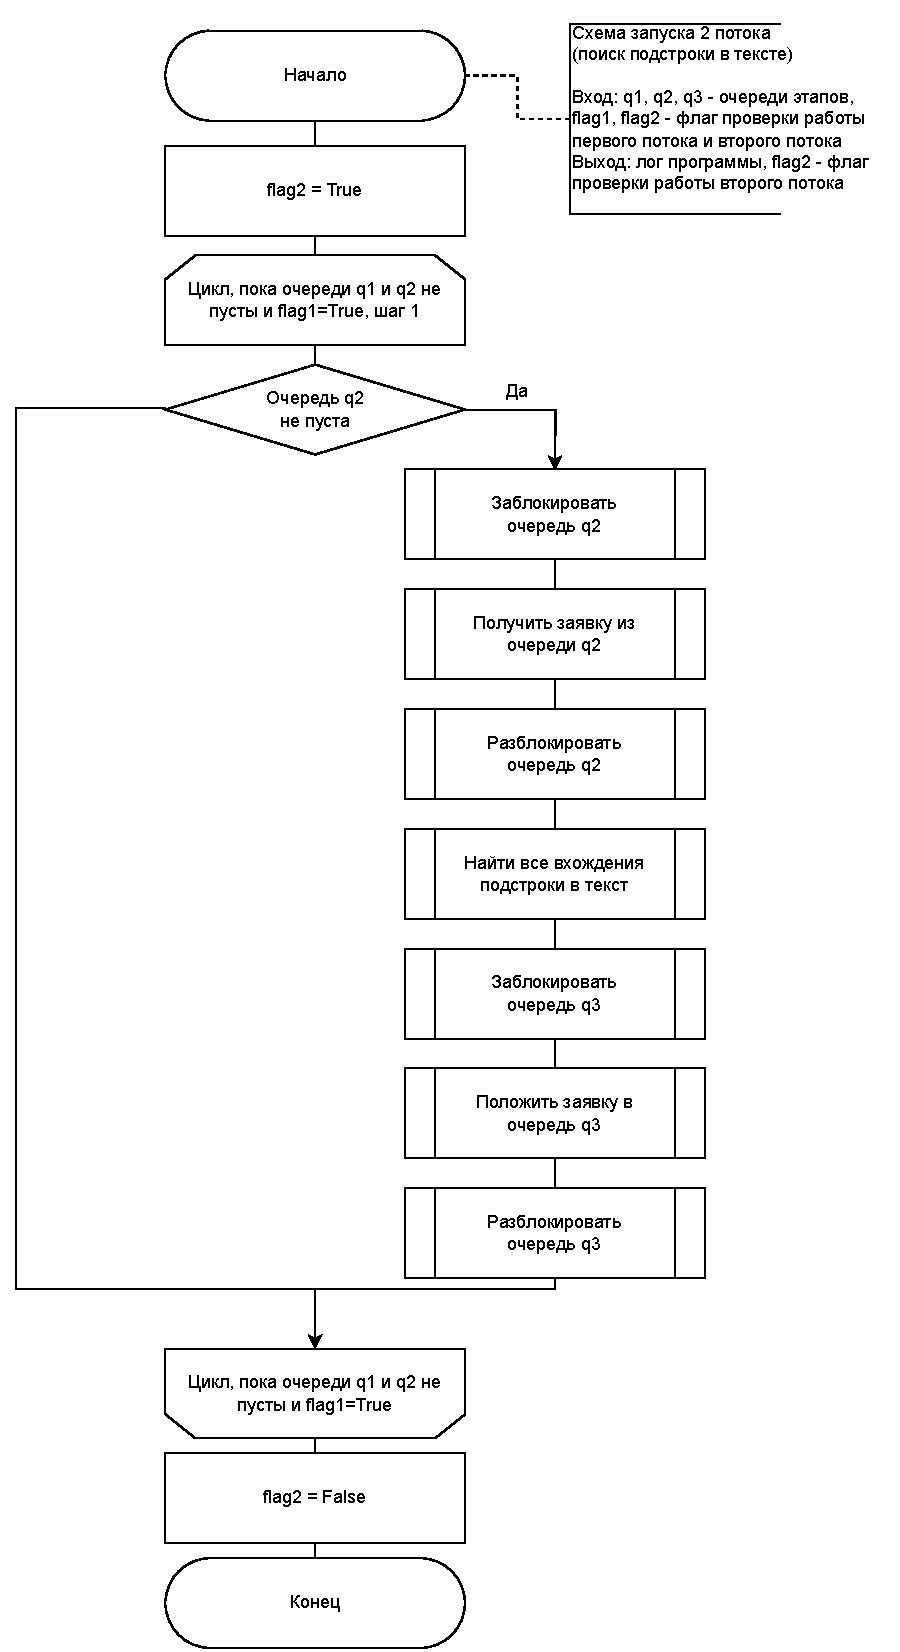
\includegraphics[scale=0.8]{photos/thread2}
	\caption{Схема алгоритма потока 2}
	\label{sh2}
\end{figure}
\clearpage

\begin{figure}[h]
	\centering
	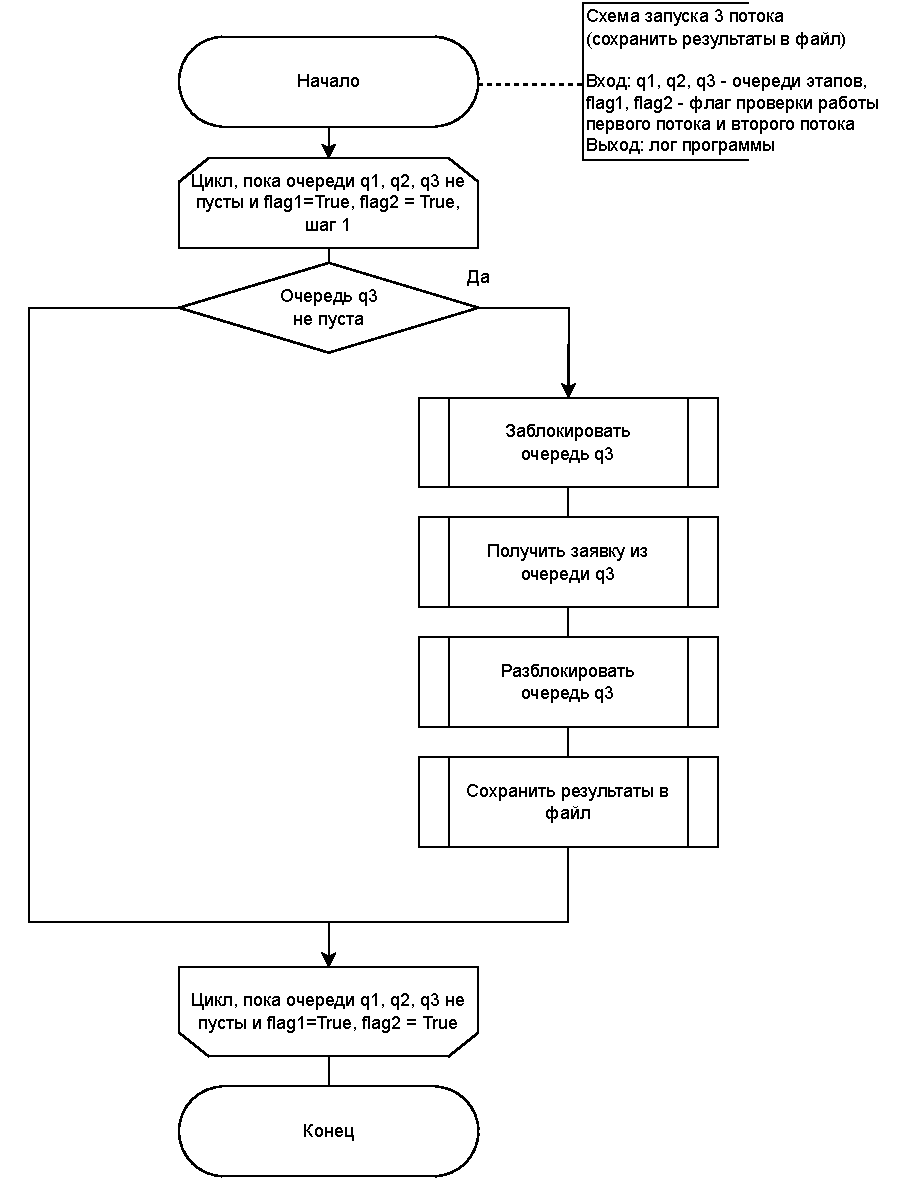
\includegraphics[scale=0.8]{photos/thread3}
	\caption{Схема алгоритма потока 3}
	\label{sh3}
\end{figure}


\section*{Вывод}

В данном разделе были представлены схемы последовательной и параллельной работы стадий конвейера.